\documentclass[a4paper]{article}

\usepackage[UTF8]{ctex}
\usepackage[a4paper,margin=1in]{geometry}
\usepackage{graphicx}
\usepackage{float}
\usepackage{listings}
\usepackage{booktabs}
\usepackage{color}
\usepackage{indentfirst}
\setlength{\parindent}{2em}
\usepackage{zhnumber}
\usepackage{adjustbox}
\usepackage{subcaption}
\usepackage{amsmath}
\usepackage{amssymb}
\usepackage{enumitem}
\usepackage{lmodern}
\usepackage{inconsolata}
\usepackage{multirow}
\usepackage{tikz}
\usetikzlibrary{positioning}
\usepackage{fancyhdr}
\usepackage{hyperref}

% 配置lstlisting支持中文
\lstset{
    language=bash, % 修改为bash或通用格式，适配交换机命令
    basicstyle=\footnotesize\ttfamily,
    breaklines=true,
    keywordstyle=\bfseries\color{blue},
    commentstyle=\itshape\color{green!50!black},
    stringstyle=\bfseries\color{red},
    numbers=left,
    numberstyle=\tiny\color{gray},
    frame=single,
    backgroundcolor=\color{gray!5},
    showstringspaces=false,
    keepspaces=true,
    tabsize=4,
    extendedchars=true,
    inputencoding=utf8,
    literate={，}{{\textcolor{green!50!black}{，}}}{1}
             {。}{{\textcolor{green!50!black}{。}}}{1}
             {：}{{\textcolor{green!50!black}{：}}}{1}
             {；}{{\textcolor{green!50!black}{；}}}{1}
             {（}{{\textcolor{green!50!black}{（}}}{1}
             {）}{{\textcolor{green!50!black}{）}}}{1}
             {【}{{\textcolor{green!50!black}{【}}}{1}
             {】}{{\textcolor{green!50!black}{】}}}{1}
}

% 根据lab8.pdf更新的基本信息
\newcommand{\projname}{计算机网络实验|实验八}
\newcommand{\reporttitle}{快速生成树协议(RSTP)配置实验个人报告}
\newcommand{\groupno}{第一组}
\newcommand{\authorname}{马福泉}
\newcommand{\major}{计算机科学与技术}
\newcommand{\adviser}{谢逸}
\newcommand{\startdate}{2025年12月7日} % 更新为PDF中的起始日期
\newcommand{\labenddate}{2025年12月20日} % 更新为PDF中的结束日期
\newcommand{\labroom}{实验D402}

\pagestyle{fancy}
\fancyhf{}
\fancyhead[L]{\kaishu \projname}
\fancyhead[C]{\kaishu \reporttitle}
\fancyhead[R]{\kaishu \authorname}
\fancyfoot[C]{第 \thepage 页}
\renewcommand{\headrulewidth}{0.4pt}
\renewcommand{\footrulewidth}{0pt}


\begin{document}

% 封面
\begin{titlepage}
    \centering
    
\includegraphics[width=10cm]{img/SYSULogo.png} % 请确保目录下有此图片，或替换图片路径
    \vspace{1em}
    \par
    {\Large \kaishu
        \par
        \projname
        \par
    }
    \vspace{3em}
    {\fontsize{40pt}{42pt}\kaishu \selectfont \boldmath \reporttitle\par}
    \vspace*{\fill}
    \begin{center}
    {\Large
    \makebox[5em][s]{姓名}:\underline{\makebox[15em][c]{\kaishu \authorname}}\\[1em]
    \makebox[5em][s]{学号}:\underline{\makebox[15em][c]{\kaishu 23336179}}\\[1em] % 请确认学号是否需要修改，此处沿用模板
    \makebox[5em][s]{小组编号}:\underline{\makebox[15em][c]{\kaishu \groupno}}\\[1em]
    \makebox[5em][s]{专业}:\underline{\makebox[15em][c]{\kaishu \major}}\\[1em]
    \makebox[5em][s]{课程教师}:\underline{\makebox[15em][c]{\kaishu \adviser}}\\[1em]
    \makebox[5em][s]{起始日期}:\underline{\makebox[15em][c]{\kaishu \startdate}}\\[1em]
    \makebox[5em][s]{结束日期}:\underline{\makebox[15em][c]{\kaishu \labenddate}}\\[1em]
    \makebox[5em][s]{实验地点}:\underline{\makebox[15em][c]{\kaishu \labroom}}
    }
    \end{center}
    \vspace*{\fill}
\end{titlepage}

\section{承担的工作}

本次快速生成树协议（RSTP）配置实验中，我参与了从基础环境搭建、环路现象观测到RSTP高级特性验证的全过程。主要承担的工作如下：

\begin{enumerate}
    \item \textbf{实验环境搭建与初始环路测试}：
    \begin{itemize}
        \item 按照实验拓扑（SwitchA与SwitchB双链路互联），协助完成了PC与交换机的物理连接及IP地址配置（PC1: 192.168.1.10, PC2: 192.168.1.20）。
        \item 在未开启STP的情况下，通过Ping操作触发了广播风暴。利用\texttt{display interface brief}命令观测到互联端口（G0/0/1, G0/0/2）利用率飙升至95\%-100\%，并结合Wireshark抓包验证了大量重复的ARP和mDNS广播包，直观确认了物理环路的危害。
    \end{itemize}

    \item \textbf{交换机基础配置与VLAN划分}：
    \begin{itemize}
        \item 协助队友将两台华为S5720交换机的基础VLAN配置，创建VLAN 10并将PC接入端口配置为Access模式。
        \item 并且配置交换机互联端口（G0/0/1-2）为Trunk模式，并允许VLAN 10通过，为后续生成树协议的部署打下基础。
    \end{itemize}

    \item \textbf{RSTP协议配置与状态验证}：
    \begin{itemize}
        \item 在两台交换机上启用RSTP模式，执行核心配置命令：
\begin{lstlisting}
stp enable
stp mode rstp
\end{lstlisting}
        \item 负责验证RSTP生效后的网络状态，观察到广播风暴消失，网络恢复正常通信。通过\texttt{display stp}命令检查全局状态，确认根桥（Root Bridge）选举结果。
        \item 负责分析端口角色与状态，确认RSTP通过阻塞冗余端口（Alternate Port, DISCARDING状态）成功打破了二层环路。
    \end{itemize}

    \item \textbf{根桥优先级控制与链路故障模拟}：
    \begin{itemize}
        \item 协助队友通过修改优先级命令\texttt{stp priority 4096}，手动指定SwitchA为根桥，验证了RSTP的根桥选举机制（优先级数值越小越优先）。
        \item 和队友一起模拟链路故障实验：断开主链路（G0/0/1），使用\texttt{ping -t}命令监测连通性。观察到网络仅出现了约4个丢包（约2秒中断）即恢复通信，验证了RSTP相比传统STP（需30-50秒）的秒级快速收敛特性。
    \end{itemize}

    \item \textbf{BPDU报文捕获与协议分析}：
    \begin{itemize}
        \item 负责分析使用Wireshark捕获RSTP的BPDU报文，详细分析了协议关键字段，包括\texttt{Root Identifier}（根桥ID）、\texttt{Bridge Identifier}（网桥ID）、\texttt{Port Role}等信息，加深了对协议交互机制的理解
    \end{itemize}
    
    \item \textbf{实验文档撰写}：
    \begin{itemize}
        \item 负责记录实验过程中的关键数据（如端口利用率变化、丢包数量），截取Wireshark抓包图及命令行输出，并主要负责撰写了本次实验的实验报告，以及后续图片的补充和排版工作。
    \end{itemize}
\end{enumerate}

\section{遇到的困难及解决方法}

在实验过程中，遇到了一些实际操作问题和理论理解上的难点，通过排查和资料查询均得以解决：

\begin{enumerate}
    \item \textbf{对华为交换机命令体系不熟悉}
    
    \textbf{现象}：在配置端口组（port-group）和Trunk端口时，部分指令与熟悉的Cisco体系不同，导致配置初期进度较慢。
    
    \textbf{解决}：查阅实验指导书及官方文档，掌握了\texttt{port-group}批量配置端口的方法，以及\texttt{display stp interface}等查看指令的正确用法，顺利完成了配置。

    \item \textbf{广播风暴现象初期不易量化观测}
    
    \textbf{现象}：在关闭STP后，虽然知道会发生环路，但仅凭肉眼观察交换机指示灯闪烁不够严谨，无法具体量化风暴的严重程度。
    
    \textbf{解决}：
    \begin{itemize}
        \item 使用\texttt{display interface brief}命令，直接观察到接口的\texttt{InUti/OutUti}（输入/输出利用率）达到了100\%，提供了确凿的数据支持。
        \item 配合Wireshark抓包，观察到同一秒内有海量重复的ARP请求（"Who has..."），从协议层面证实了二层环路导致的数据帧无限复制。
    \end{itemize}

    \item \textbf{RSTP收敛时间的精确捕捉}
    
    \textbf{现象}：RSTP收敛速度极快（秒级），在模拟拔线故障时，操作不同步很容易错过丢包瞬间，难以直观对比出与STP的区别。
    
    \textbf{解决}：采用“持续Ping”策略。在PC端预先执行\texttt{ping 192.168.1.20 -t}，保持数据流不断。然后由队友物理断开网线，我紧盯着屏幕记录“请求超时”的次数。最终准确记录下丢失了4个包，推算出大概的收敛时间，验证了RSTP的快速特性。

    
    \item \textbf{广播风暴形成时间的精确统计}
    \textbf{遇到的困难}：在对比“Ping正常IP”与“Ping不存在IP”的包增长速率时，难以通过交换机命令行精确记录达到饱和的具体秒数。

    % 插入截图并说明
    \begin{figure}[H]
        \centering
        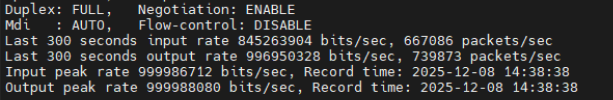
\includegraphics[width=0.8\textwidth]{img/problem.png}
        \caption{交换机命令行观测端口流量利用率时的实际截图。可以看到，统计数据显示的是过去一段时间（如300秒）的平均值，难以精确捕捉广播风暴流量突增的具体时刻。}
        \label{fig:problem}
    \end{figure}

    \textbf{原因分析}：
    \begin{itemize}
        \item \textbf{统计采样间隔限制}：实验设备（S5720）的接口流量利用率统计（InUti/OutUti）通常显示的是过去一段时间（如300秒）的平均值。广播风暴属于毫秒级的瞬间突发流量，交换机的平均算法“平滑”了瞬时峰值，导致无法通过CLI直接观测到流量从0激增到100\%的精确时间点。
        \item \textbf{控制平面拥塞}：在触发广播风暴（特别是Ping不存在IP导致ARP泛洪）时，交换机CPU利用率急剧升高，命令行终端响应迟缓，无法进行实时的高频刷新观测。
    \end{itemize}

    \textbf{解决方法/替代方案}：改为使用人为计时端口流量利用率上升速度，并且配合Wireshark抓包工具进行分析。
    \begin{itemize}
        \item 情况一（Ping正常IP）：数据包时间间隔相对稳定，流量增长呈线性。
        \item 情况二（Ping不存在IP）：在极短时间内出现大量重复的ARP广播包，时间戳高度重叠，从而证明了该情况下流量呈指数级爆炸增长，迅速导致网络饱和。
    \end{itemize}

    \textbf{补充说明}：虽然可以通过命令\texttt{set flow-stat interval 10}将统计间隔修改为更短时间（如10秒），但在广播风暴的极端负载下，此操作意义不大
\end{enumerate}

\section{体会与总结}

本次实验通过对比未启用生成树协议时的网络瘫痪状态与启用RSTP后的稳定运行，让我对二层网络冗余技术有了深刻的理解：

\begin{itemize}
    \item \textbf{深刻认识了二层环路的危害}：实验中直观看到的100\%端口利用率和指数级增长的广播包，让我明白了物理冗余虽然提供了备份，但如果没有逻辑上的防环机制（如STP），反而会导致网络不可用。广播风暴和MAC地址表震荡是二层网络的致命问题。
    
    \item \textbf{掌握了RSTP的核心机制}：通过手动修改优先级控制根桥选举，以及观察端口状态从\texttt{Discarding}变为\texttt{Forwarding}的过程，我实际验证了RSTP的端口角色（根端口、指定端口、备用端口）分配逻辑。理解了它是如何通过阻塞特定端口来构建无环逻辑拓扑的。
    
    \item \textbf{验证了“快速”生成的实际意义}：通过链路故障切换测试，亲眼见证了网络在2秒内自动恢复。对比理论知识中传统STP需要30-50秒的恢复时间，深刻体会到了RSTP（802.1w）引入P/A机制和边缘端口等改进对提升现代网络高可用性的重要价值。
    
    \item \textbf{提升了网络排错与分析能力}：在实验中综合使用了命令行状态查询（\texttt{display}）、链路流量监控和Wireshark协议分析等多种手段，这种多维度的分析方法对于今后解决复杂的网络工程问题大有裨益。
\end{itemize}

\end{document}